\documentclass[10pt]{article}
\newcommand\tab[1][.5cm]{\hspace*{#1}}
\usepackage{graphicx}
\graphicspath{ {images/} }

\begin{document}

\title{Homework 5 - Sorting Algorithms}
\author{Michael Gould\\ 
CS 288 - Intensive Programming in Linux}

\maketitle

The following graphs show the performance of each of the three different kinds of sorting algorithms in ascending order of efficacy.

\center
\huge
\textbf{Selection Sort}
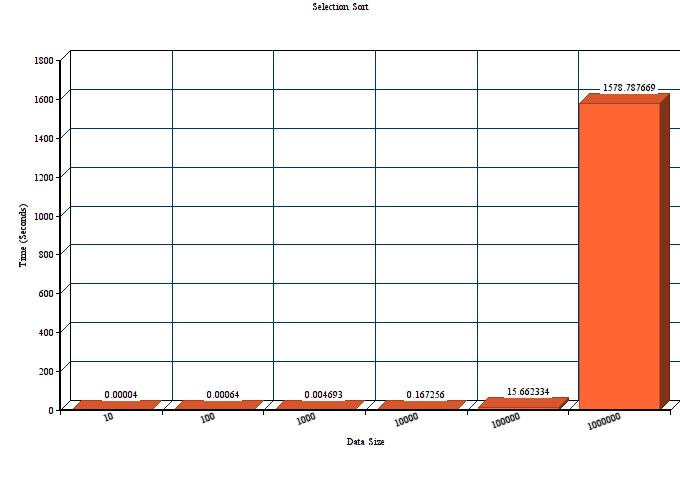
\includegraphics[scale=0.6]{Select.jpg}

\textbf{Merge Sort}
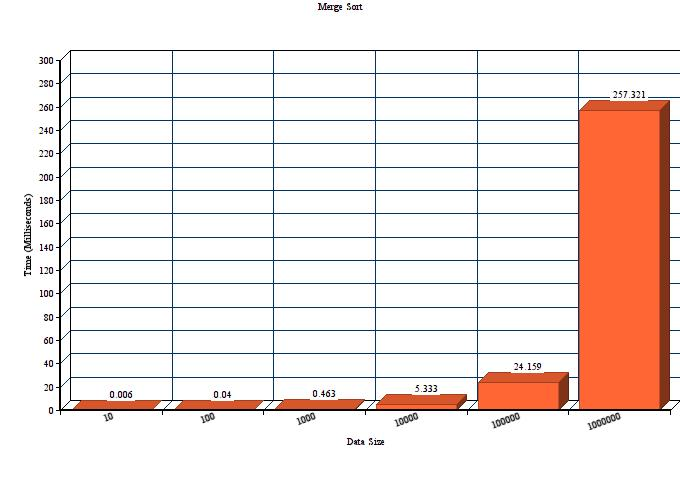
\includegraphics[scale=0.6]{Merge.jpg}

\textbf{Radix Sort}
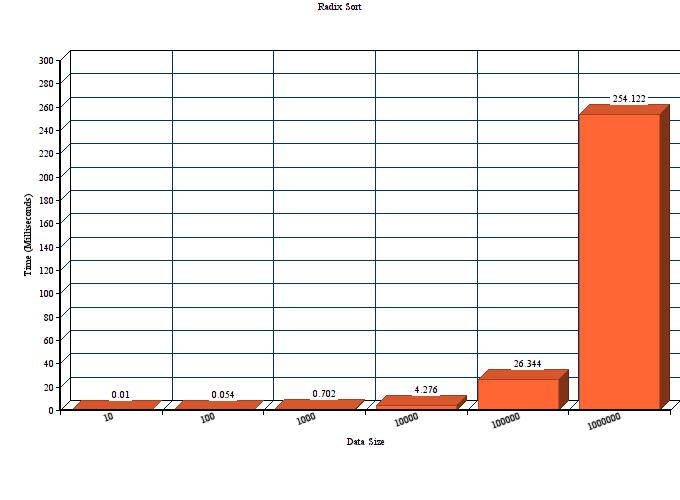
\includegraphics[scale=0.6]{Radix.jpg}

\normalsize
\flushleft



\tab The first algorithm listed is Selection Sort, which iterates through the entirety of an array finding the outlying value (minimum or maximum) of an unsorted array and places it into the correct position of a sorted array.  Given the complexities of iterating through two separate arrays, the time complexity is that of $n^2$.  It is worth mentioning that to cohesively compose the graph shown, it was necessary to use the unit "seconds" to properly express the output, especially in the upper bounds of 100K elements and 1M elements.\\

\tab The second of these algorithms was that of a Merge Sort.  A merge sort is accomplished by finding the middle of an array and subdividing it into to arrays of half the initial size.  This process is then repeated until the last array can no longer be split to a size any smaller since it is of one element in length.  This path is then traversed backwards and each array is merged with a corresponding branch, in order by value.  It can be thought of as a binary tree, with each child leaf being an array of half the size of the parent leaf until the last leaf is that of an array of size 1.  The speed of such a process is far greater than that of the selection sort and thus required a manipulation of the graph's time to be represented by that of "milliseconds" rather than "seconds".  This is due to the fact that the time complexity of the algorithm is $n \log n$.  A noteworthy finding of this algorithm is that given any array, the results are always $n \log n$ no matter the input array.  This is of particular interest, since in many cases, input data to an array is not controlled by the programmer and therefore can create inconsistency, but with this algorithm you are assured that no matter the input, the results will always be that of $n \log n$.\\

\tab The last of these algorithms was one called Radix Sort.  This algorithm is accomplished through the organization of each sub-variable of data into bins ordered by all the variations of said data.  The test used was on an array of integers, so each element was compared by its cooresponding digit value and placed into bins of each possibility (numbers 0-9) before being concatenated thereafter into a second array of the same size, with the process being repeated for the following digit, up to the highest existing digit value in the input data set.  This means that the speed of the sort cooresponds to that of the number of digit values found in the input, for example a set of 1 million integers between the values of 0-999 would only be sent into these sub arrays 3 times, one of the ones digit, one for the tens digit and finally one for the hundreds digit.  While this is very impressive for input data that limits its digit values, with larger values the sort begins to behave closely to that of the merge sort due to the distinct differences is word length. This algorithm is said to have a time complexity of that of $n$, but in reality this is actually $nw$ where $w$ is word length.
\end{document}
